\documentclass[a4paper]{article}

\usepackage{amsmath}
\usepackage{hyperref}
\usepackage{graphicx}
\usepackage{float}

\title{Using local binary patterns to read license plates in photographs}

% Paragraph indentation
\setlength{\parindent}{0pt}
\setlength{\parskip}{1ex plus 0.5ex minus 0.2ex}

\begin{document}
\maketitle

\section*{Project members}
Gijs van der Voort\\
Richard Torenvliet\\
Jayke Meijer\\
Tadde\"us Kroes\\
Fabi\'en Tesselaar

\tableofcontents
\pagebreak

\setcounter{secnumdepth}{1}

\section{Problem description}

License plates are used for uniquely identifying motorized vehicles and are
made to be read by humans from great distances and in all kinds of weather
conditions.

Reading license plates with a computer is much more difficult. Our dataset
contains photographs of license plates from various angles and distances. This
means that not only do we have to implement a method to read the actual
characters, but given the location of the license plate and each individual
character, we must make sure we transform each character to a standard form. 

Determining what character we are looking at will be done by using Local Binary
Patterns. The main goal of our research is finding out how effective LBP's are
in classifying characters on a license plate.

In short our program must be able to do the following:

\begin{enumerate}
    \item Extracting characters using the location points in the xml file.
    \item Reduce noise where possible to ensure maximum readability.
    \item Transforming a character to a normal form.
    \item Creating a local binary pattern histogram vector.
    \item Matching the found vector with a learning set.
    \item And finally it has to check results with a real data set.
\end{enumerate}

\section{Language of choice}

The actual purpose of this project is to check if LBP is capable of recognizing
license plate characters. We knew the LBP implementation would be pretty
simple. Thus an advantage had to be its speed compared with other license plate 
recognition implementations, but the uncertainty of whether we could get some
results made us pick Python. We felt Python would not restrict us as much in 
assigning tasks to each member of the group. In addition, when using the
correct modules to handle images, Python can be decent in speed.

\section{Theory}

Now we know what our program has to be capable of, we can start with the
defining what problems we have and how we want to solve these.

\subsection{Extracting a letter and resizing it}

Rewrite this section once we have implemented this properly.
%NO LONGER VALID!
%Because we are already given the locations of the characters, we only need to
%transform those locations using the same perspective transformation used to
%create a front facing license plate. The next step is to transform the
%characters to a normalized manner. The size of the letter W is used as a
%standard to normalize the width of all the characters, because W is the widest
%character of the alphabet. We plan to also normalize the height of characters,
%the best manner for this is still to be determined.

%\begin{enumerate}
%    \item Crop the image in such a way that the character precisely fits the
%          image.
%    \item Scale the image to a standard height.
%    \item Extend the image on either the left or right side to a certain width.
%\end{enumerate}

%The resulting image will always have the same size, the character contained
%will always be of the same height, and the character will always be positioned
%at either the left of right side of the image.

\subsection{Transformation}

A simple perspective transformation will be sufficient to transform and resize
the characters to a normalized format. The corner positions of characters in
the dataset are supplied together with the dataset.

\subsection{Reducing noise}

Small amounts of noise will probably be suppressed by usage of a Gaussian
filter. A real problem occurs in very dirty license plates, where branches and
dirt over a letter could radically change the local binary pattern. A question
we can ask ourselves here, is whether we want to concentrate ourselves on these
exceptional cases. By law, license plates have to be readable. However, the
provided dataset showed that this does not mean they always are. We will have
to see how the algorithm performs on these plates, however we have good hopes
that our method will get a good score on dirty plates, as long as a big enough
part of the license plate remains readable.

\subsection{Local binary patterns}
Once we have separate digits and characters, we intent to use Local Binary
Patterns (Ojala, Pietikäinen \& Harwood, 1994) to determine what character
or digit we are dealing with. Local Binary
Patterns are a way to classify a texture based on the distribution of edge
directions in the image. Since letters on a license plate consist mainly of
straight lines and simple curves, LBP should be suited to identify these.

\subsubsection{LBP Algorithm}
The LBP algorithm that we implemented can use a variety of neighbourhoods,
including the same square pattern that is introduced by Ojala et al (1994),
and a circular form as presented by Wikipedia.
\begin{itemize}
\item Determine the size of the square where the local patterns are being
registered. For explanation purposes let the square be 3 x 3. \\
\item The grayscale value of the middle pixel is used as threshold. Every
value of the pixel around the middle pixel is evaluated. If it's value is
greater than the threshold it will be become a one else a zero.

\begin{figure}[h!]
\center
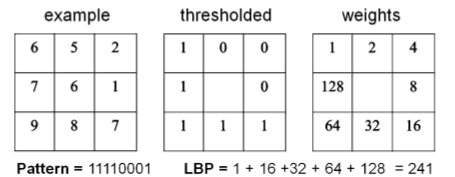
\includegraphics[scale=0.5]{lbp.png}
\caption{LBP 3 x 3 (Pietik\"ainen, Hadid, Zhao \& Ahonen (2011))}
\end{figure}

Notice that the pattern will be come of the form 01001110. This is done when a
the value of the evaluated pixel is greater than the threshold, shift the bit
by the n(with i=i$_{th}$ pixel evaluated, starting with $i=0$).

This results in a mathematical expression:

Let I($x_i, y_i$) an Image with grayscale values and $g_n$ the grayscale value
of the pixel $(x_i, y_i)$. Also let $s(g_i, g_c)$ (see below) with $g_c$ =
grayscale value of the center pixel and $g_i$ the grayscale value of the pixel
to be evaluated.

$$
  s(g_i, g_c) = \left\{
  \begin{array}{l l}
    1 & \quad \text{if $g_i$ $\geq$ $g_c$}\\
    0 & \quad \text{if $g_i$ $<$ $g_c$}\\
  \end{array} \right.
$$

$$LBP_{n, g_c = (x_c, y_c)} = \sum\limits_{i=0}^{n-1} s(g_i, g_c)^{2i} $$

The outcome of this operations will be a binary pattern.

\item Given this pattern, the next step is to divide the pattern in cells. The
amount of cells depends on the quality of the result, so trial and error is in
order. Starting with dividing the pattern in to cells of size 16. 

\item Compute a histogram for each cell.

\begin{figure}[h!]
\center
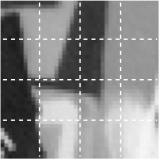
\includegraphics[scale=0.7]{cells.png}
\caption{Divide in cells(Pietik\"ainen et all (2011))}
\end{figure}

\item Consider every histogram as a vector element and concatenate these. The
result is a feature vector of the image.

\item Feed these vectors to a support vector machine. This will ''learn'' which
vector indicates what vector is which character. 

\end{itemize}

To our knowledge, LBP has yet not been used in this manner before. Therefore,
it will be the first thing to implement, to see if it lives up to the
expectations. When the proof of concept is there, it can be used in a final
program.

Later we will show that taking a histogram over the entire image (basically
working with just one cell) gives us the best results.

\subsection{Matching the database}

Given the LBP of a character, a Support Vector Machine can be used to classify
the character to a character in a learning set. The SVM uses a concatenation
of each cell in an image as a feature vector (in the case we check the entire
image no concatenation has to be done of course. The SVM can be trained with a
subset of the given dataset called the ''Learning set''. Once trained, the
entire classifier can be saved as a Pickle object\footnote{See
\url{http://docs.python.org/library/pickle.html}} for later usage.
In our case the support vector machine uses a radial gauss kernel. The SVM finds
a seperating hyperplane with minimum margins.

\section{Implementation}

In this section we will describe our implementations in more detail, explaining
choices we made.

\subsection{Character retrieval}

In order to retrieve the characters from the entire image, we need to
perform a perspective transformation. However, to do this, we need to know the 
coordinates of the four corners of each character. For our dataset, this is
stored in XML files. So, the first step is to read these XML files.

\paragraph*{XML reader}

The XML reader will return a 'license plate' object when given an XML file. The
licence plate holds a list of, up to six, NormalizedImage characters and from
which country the plate is from. The reader is currently assuming the XML file
and image name are corresponding, since this was the case for the given
dataset. This can easily be adjusted if required. 

To parse the XML file, the minidom module is used. So the XML file can be
treated as a tree, where one can search for certain nodes. In each XML
file it is possible that multiple versions exist, so the first thing the reader
will do is retrieve the current and most up-to-date version of the plate. The
reader will only get results from this version.

Now we are only interested in the individual characters so we can skip the
location of the entire license plate. Each character has 
a single character value, indicating what someone thought what the letter or
digit was and four coordinates to create a bounding box. If less then four points have been set the character will not be saved. Else, to make things not to
complicated, a Character class is used. It acts as an associative list, but it gives some extra freedom when using the
data.

When four points have been gathered the data from the actual image is being
requested. For each corner a small margin is added (around 3 pixels) so that no
features will be lost and minimum amounts of new features will be introduced by
noise in the margin. 

In the next section you can read more about the perspective transformation that
is being done. After the transformation the character can be saved: Converted
to grayscale, but nothing further. This was used to create a learning set. If
it does not need to be saved as an actual image it will be converted to a
NormalizedImage. When these actions have been completed for each character the
license plate is usable in the rest of the code.

\paragraph*{Perspective transformation}
Once we retrieved the corner points of the character, we feed those to a
module that extracts the (warped) character from the original image, and
creates a new image where the character is cut out, and is transformed to a
rectangle.

\subsection{Noise reduction}

The image contains a lot of noise, both from camera errors due to dark noise 
etc., as from dirt on the license plate. In this case, noise therefore means 
any unwanted difference in color from the surrounding pixels.

\paragraph*{Camera noise and small amounts of dirt}
The dirt on the license plate can be of different sizes. We can reduce the 
smaller amounts of dirt in the same way as we reduce normal noise, by applying
a Gaussian blur to the image. This is the next step in our program.\\
\\
The Gaussian filter we use comes from the \texttt{scipy.ndimage} module. We use
this function instead of our own function, because the standard functions are
most likely more optimized then our own implementation, and speed is an
important factor in this application.

\paragraph*{Larger amounts of dirt}
Larger amounts of dirt are not going to be resolved by using a Gaussian filter.
We rely on one of the characteristics of the Local Binary Pattern, only looking
at the difference between two pixels, to take care of these problems.\\
Because there will probably always be a difference between the characters and
the dirt, and the fact that the characters are very black, the shape of the
characters will still be conserved in the LBP, even if there is dirt
surrounding the character.

\subsection{Creating Local Binary Patterns and feature vector}
Every pixel is a center pixel and it is also a value to evaluate but not at the 
same time. Every pixel is evaluated as shown in the explanation
of the LBP algorithm. There are several neighbourhoods we can evaluate. We have
tried the following neighbourhoods:

\begin{figure}[H]
\center
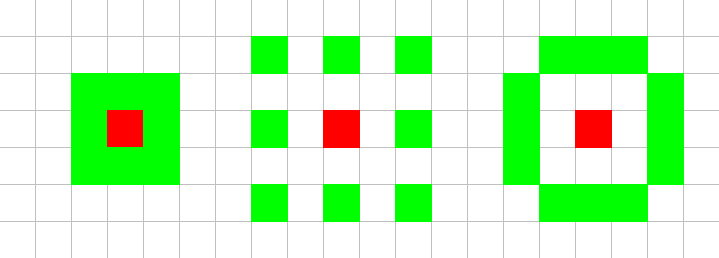
\includegraphics[scale=0.5]{neighbourhoods.png}
\caption{Tested neighbourhoods}
\end{figure}

We chose these neighbourhoods to prevent having to use interpolation, which
would add a computational step, thus making the code execute slower. In the
next section we will describe what the best neighbourhood was.

Take an example where the full square can be evaluated, so none of the
neighbours are out of bounds. The first to be checked is the pixel in the left 
bottom corner in the square 3 x 3, with coordinate $(x - 1, y - 1)$ with $g_c$ 
as center pixel that has coordinates $(x, y)$. If the grayscale value of the
neighbour in the left corner is greater than the grayscale
value of the center pixel than return true. Bit-shift the first bit with 7. The
outcome is now 1000000. The second neighbour will be bit-shifted with 6, and so 
on. Until we are at 0. The result is a binary pattern of the local point just
evaluated.
Now only the edge pixels are a problem, but a simple check if the location of
the neighbour is still in the image can resolve this. We simply state that the
pixel has a lower value then the center pixel if it is outside the image
bounds.

\paragraph*{Histogram and Feature Vector}
After all the Local Binary Patterns are created for every pixel, this pattern
is divided into cells. The feature vector is the vector of concatenated
histograms. These histograms are created for cells. These cells are created by
dividing the \textbf{pattern} in to cells and create a histogram of that. So
multiple cells are related to one histogram. All the histograms are
concatenated and fed to the SVM that will be discussed in the next section,
Classification. We did however find out that the use of several cells was not
increasing our performance, so we only have one histogram to feed to the SVM.

\subsection{Classification}

For the classification, we use a standard Python Support Vector Machine,
\texttt{libsvm}. This is a often used SVM, and should allow us to simply feed
the data from the LBP and Feature Vector steps into the SVM and receive results.\\
\\
Using a SVM has two steps. First you have to train the SVM, and then you can
use it to classify data. The training step takes a lot of time, so luckily
\texttt{libsvm} offers us an opportunity to save a trained SVM. This means,
you do not have to train the SVM every time.

\section{Finding parameters}

Now that we have a functioning system, we need to tune it to work properly for
license plates. This means we need to find the parameters. Throughout the 
program we have a number of parameters for which no standard choice is
available. These parameters are:\\
\\
\begin{tabular}{l|l}
	Parameter 			& Description\\
	\hline
	$\sigma$  			& The size of the Gaussian blur.\\
	\emph{cell size}	& The size of a cell for which a histogram of LBP's
	                      will be generated.\\
	\emph{Neighbourhood}& The neighbourhood to use for creating the LBP.\\
	$\gamma$			& Parameter for the Radial kernel used in the SVM.\\
	$c$					& The soft margin of the SVM. Allows how much training
						  errors are accepted.\\
\end{tabular}\\
\\
For each of these parameters, we will describe how we searched for a good
value, and what value we decided on.

\subsection{Parameter $\sigma$}

The first parameter to decide on, is the $\sigma$ used in the Gaussian blur. To
find this parameter, we tested a few values, by trying them and checking the
results. It turned out that the best value was $\sigma = 1.4$.

\subsection{Parameter \emph{cell size}}

The cell size of the Local Binary Patterns determines over what region a
histogram is made. The trade-off here is that a bigger cell size makes the
classification less affected by relative movement of a character compared to
those in the learning set, since the important structure will be more likely to
remain in the same cell. However, if the cell size is too big, there will not
be enough cells to properly describe the different areas of the character, and
the feature vectors will not have enough elements.\\
\\
In order to find this parameter, we used a trial-and-error technique on a few
cell sizes. During this testing, we discovered that a lot better score was
reached when we take the histogram over the entire image, so with a single
cell. Therefore, we decided to work without cells.\\
\\
A reason we can think of why using one cell works best is that the size of a
single character on a license plate in the provided dataset is very small.
That means that when dividing it into cells, these cells become simply too
small to have a really representative histogram. Therefore, the
concatenated histograms are then a list of only very small numbers, which
are not significant enough to allow for reliable classification.

\subsection{Parameter \emph{Neighbourhood}}

The neighbourhood to use can only be determined through testing. We did a test
with each of these neighbourhoods, and we found that the best results were
reached with the following neighbourhood, which we will call the
(12, 5)-neighbourhood, since it has 12 points in a area with a diameter of 5.

\begin{figure}[H]
\center
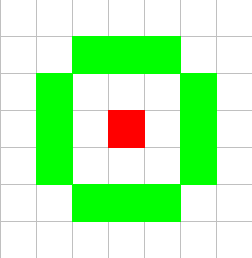
\includegraphics[scale=0.5]{12-5neighbourhood.png}
\caption{(12,5)-neighbourhood}
\end{figure}

\subsection{Parameters $\gamma$ \& $c$}

The parameters $\gamma$ and $c$ are used for the SVM. $c$ is a standard
parameter for each type of SVM, called the 'soft margin'. This indicates how
exact each element in the learning set should be taken. A large soft margin
means that an element in the learning set that accidentally has a completely
different feature vector than expected, due to noise for example, is not taken
into account. If the soft margin is very small, then almost all vectors will be
taken into account, unless they differ extreme amounts.\\
$\gamma$ is a variable that determines the size of the radial kernel, and as
such determines how steep the difference between two classes can be.\\
\\
Since these parameters both influence the SVM, we need to find the best
combination of values. To do this, we perform a so-called grid-search. A
grid-search takes exponentially growing sequences for each parameter, and
checks for each combination of values what the score is. The combination with
the highest score is then used as our parameters, and the entire SVM will be
trained using those parameters.\\
\\
The results of this grid-search are shown in the following table. The values
in the table are rounded percentages, for easy displaying.

\begin{tabular}{|r|r r r r r r r r r r|}
\hline
c $\gamma$ & $2^{-15}$ & $2^{-13}$ & $2^{-11}$ & $2^{-9}$ & $2^{-7}$ &
	$2^{-5}$ & $2^{-3}$ & $2^{-1}$ & $2^{1}$ & $2^{3}$\\
\hline
$2^{-5}$ &       61 &       61 &       61 &       61 &       62 &
       63 &       67 &       74 &       59 &       24\\
$2^{-3}$ &       61 &       61 &       61 &       61 &       62 &
       63 &       70 &       78 &       60 &       24\\
$2^{-1}$ &       61 &       61 &       61 &       61 &       62 &
       70 &       83 &       88 &       78 &       27\\
 $2^{1}$ &       61 &       61 &       61 &       61 &       70 &
        84 &       90 &       92 &       86 &       45\\
 $2^{3}$ &       61 &       61 &       61 &       70 &       84 &
        90 &       93 &       93 &       86 &       45\\
 $2^{5}$ &       61 &       61 &       70 &       84 &       90 &
        92 &       93 &       93 &       86 &       45\\
 $2^{7}$ &       61 &       70 &       84 &       90 &       92 &
        93 &       93 &       93 &       86 &       45\\
 $2^{9}$ &       70 &       84 &       90 &       92 &       92 & 
       93 &       93 &       93 &       86 &       45\\
$2^{11}$ &       84 &       90 &       92 &       92 &       92 &
       92 &       93 &       93 &       86 &       45\\
$2^{13}$ &       90 &       92 &       92 &       92 &       92 &
       92 &       93 &       93 &       86 &       45\\
$2^{15}$ &       92 &       92 &       92 &       92 &       92 &
       92 &       93 &       93 &       86 &       45\\
\hline
\end{tabular}

We found that the best values for these parameters are $c = 32$ and
$\gamma = 0.125$.

\section{Results}

The goal was to find out two things with this research: The speed of the
classification and the accuracy. In this section we will show our findings.

\subsection{Speed}

Recognizing license plates is something that has to be done fast, since there
can be a lot of cars passing a camera in a short time, especially on a highway.
Therefore, we measured how well our program performed in terms of speed. We
measure the time used to classify a license plate, not the training of the
dataset, since that can be done offline, and speed is not a primary necessity
there.\\
\\
The speed of a classification turned out to be reasonably good. We time between
the moment a character has been 'cut out' of the image, so we have a exact
image of a character, to the moment where the SVM tells us what character it is.
This time is on average $65$ ms. That means that this
technique (tested on an AMD Phenom II X4 955 Quad core CPU running at 3.2 GHz)
can identify 15 characters per second.\\
\\
This is not spectacular considering the amount of calculating power this cpu
can offer, but it is still fairly reasonable. Of course, this program is
written in Python, and is therefore not nearly as optimized as would be
possible when written in a low-level language.

\subsection{Accuracy}

Of course, it is vital that the recognition of a license plate is correct,
almost correct is not good enough here. Therefore, we have to get the highest
accuracy score we possibly can.\\
\\ According to Wikipedia
\footnote{
\url{http://en.wikipedia.org/wiki/Automatic_number_plate_recognition}},
commercial license plate recognition software score about $90\%$ to $94\%$,
under optimal conditions and with modern equipment.\\
\\
Our program scores an average of $93\%$. However, this is for a single
character. That means that a full license plate should theoretically
get a score of $0.93^6 = 0.647$, so $64.7\%$. That is not particularly
good compared to the commercial ones. However, our focus was on getting
good scores per character, and $93\%$ seems to be a fairly good result.\\
\\
Possibilities for improvement of this score would be more extensive
grid-searches, finding more exact values for $c$ and $\gamma$, more tests
for finding $\sigma$ and more experiments on the size and shape of the 
neighbourhoods.

\section{Conclusion}

In the end it turns out that using Local Binary Patterns is a promising
technique for License Plate Recognition. It seems to be relatively indifferent
for the amount of dirt on license plates and different fonts on these plates.\\
\\
The performance speed wise is fairly good, when using a fast machine. However,
this is written in Python, which means it is not as efficient as it could be
when using a low-level languages.
\\
We believe that with further experimentation and development, LBP's can
absolutely be used as a good license plate recognition method.

\section{Reflection}

\subsection{Difficulties}

During the implementation and testing of the program, we did encounter a
number of difficulties. In this section we will state what these difficulties
were and whether we were able to find a proper solution for them.

\subsubsection*{Dataset}

We did experience a number of problems with the provided dataset. A number of
these are problems to be expected in a real world problem, but which make
development harder. Others are more elemental problems.\\
The first problem was that the dataset contains a lot of license plates which
are problematic to read, due to excessive amounts of dirt on them. Of course,
this is something you would encounter in the real situation, but it made it
hard for us to see whether there was a coding error or just a bad example.\\
Another problem was that there were license plates of several countries in
the dataset. Each of these countries has it own font, which also makes it
hard to identify these plates, unless there are a lot of these plates in the
learning set.\\
A problem that is more elemental is that some of the characters in the dataset
are not properly classified. This is of course very problematic, both for
training the SVM as for checking the performance. This meant we had to check
each character whether its description was correct.

\subsubsection*{SVM}

We also had trouble with the SVM for Python. The standard Python SVM, libsvm,
had a poor documentation. There was no explanation what so ever on which
parameter had to be what. This made it a lot harder for us to see what went
wrong in the program.

\subsection{Workload distribution}

The first two weeks were team based. Basically the LBP algorithm could be
implemented in the first hour, while some talked and someone did the typing.
Some additional 'basics' where created in similar fashion. This ensured that
every team member was up-to-date and could start figuring out which part of the
implementation was most suited to be done by one individually or in a pair.

\subsubsection*{Who did what}
Gijs created the basic classes we could use and helped the rest everyone by 
keeping track of what required to be finished and whom was working on what. 
Tadde\"us and Jayke were mostly working on the SVM and all kinds of tests
whether the histograms were matching and alike. Fabi\"en created the functions
to read and parse the given xml files with information about the license
plates. Upon completion all kinds of learning and data sets could be created.
Richard helped out wherever anyone needed a helping hand, and was always
available when someone had to talk or ask something.

\subsubsection*{How it went}

Sometimes one cannot hear the alarm bell and wake up properly. This however was
not a big problem as no one was afraid of staying at Science Park a bit longer
to help out. Further communication usually went through e-mails and replies
were instantaneous! A crew to remember.

\end{document}
